\documentclass[12pt, a4paper]{article}

% --- Packages ---
\usepackage[margin=2.5cm]{geometry}
\usepackage{graphicx}
\usepackage{hyperref}
\usepackage{xcolor}
\usepackage{enumitem}
\usepackage{booktabs}
\usepackage{tikz}
\usetikzlibrary{shapes.geometric, arrows.meta, positioning, fit, backgrounds, calc}
\usepackage{float}
\usepackage{listings}
\usepackage{fancyhdr}
\usepackage[T1]{fontenc}
\usepackage{lmodern}
\usepackage{titlesec}

% --- Page Style ---
\pagestyle{fancy}
\fancyhf{}
\rhead{\textit{SmartHVAC Studio}}
\lhead{\textit{ME420 Research Project}}
\rfoot{Page \thepage}

% --- Section Numbering Depth ---
\setcounter{secnumdepth}{4}
\setcounter{tocdepth}{3}

% --- Paragraph-level numbering format ---
\titleformat{\paragraph}[hang]{\normalfont\normalsize\bfseries}{\theparagraph}{1em}{}
\titlespacing*{\paragraph}{0pt}{2.5ex plus 1ex minus .2ex}{0.5ex plus .2ex}

% --- Code Listing Style ---
\lstset{
  basicstyle=\ttfamily\small,
  keywordstyle=\color{blue}\bfseries,
  commentstyle=\color{gray},
  stringstyle=\color{red!70!black},
  breaklines=true,
  frame=single,
  numbers=none,
  backgroundcolor=\color{gray!5},
  rulecolor=\color{gray!40},
}

% --- Colours ---
\definecolor{layerblue}{HTML}{1a73e8}
\definecolor{layergreen}{HTML}{0d904f}

\hypersetup{
  colorlinks=true,
  linkcolor=layerblue,
  urlcolor=layerblue,
  citecolor=layerblue,
}

% ==============================================================================
\begin{document}

\begin{titlepage}
  \centering
  \vspace*{3cm}
  {\Huge\bfseries SmartHVAC Studio\\[0.4cm]}
  {\Large\itshape Project Architecture \& System Documentation\\[1.5cm]}
  {\large ME420 --- Mechanical Engineering Research Project\\[0.3cm]}
  {\large Department of Mechanical Engineering\\[0.3cm]}
  {\large University of Moratuwa\\[2cm]}
  \rule{0.6\textwidth}{0.4pt}\\[1cm]
  {\large\today}
  \vfill
\end{titlepage}

\tableofcontents
\newpage

% ==============================================================================
\section{Introduction}
% ==============================================================================

SmartHVAC Studio is a cloud-based research platform that enables users to generate and simulate building energy models through natural language descriptions. A user describes a building in plain English (e.g.,\ ``Create a 15$\times$15 building with brick walls''), and the system autonomously produces a valid EnergyPlus Input Data File (IDF), executes the thermal simulation on a GPU-equipped Google Colab runtime, and returns time-series result plots to a web dashboard.

The platform is designed around a \textbf{5-Layer Architecture} in which the Web Frontend, Firebase Cloud Services, a Colab Backend Worker, an Agentic AI Pipeline, and the EnergyPlus Simulation Engine each operate as independent, loosely coupled layers. This document explains every layer, every source file, and the data flow that connects them.

% ==============================================================================
\section{Repository Structure}
% ==============================================================================

The two primary directories are \texttt{web/} (Layer~1) and \texttt{colab/} (Layers~3--5). Their contents are summarised below.

\begin{table}[h!]
\centering
\caption{Key files in the \texttt{web/} directory (Layer 1).}
\label{tab:web}
\small
\begin{tabular}{@{}llp{7.0cm}@{}}
\toprule
\textbf{File} & \textbf{Type} & \textbf{Purpose} \\
\midrule
\texttt{index.html}          & HTML  & Landing page with navigation sidebar. \\
\texttt{pages/nlp.html}      & HTML  & Simulation Setup form: text area, model selector, weather file picker. \\
\texttt{pages/results.html}  & HTML  & Job history table, result plots, View IDF and View Object Summary buttons. \\
\texttt{pages/idf\_viewer.html} & HTML & Standalone IDF text viewer. \\
\texttt{pages/architecture.html} & HTML & In-app architecture diagram page. \\
\texttt{script.js}           & JS    & All client logic: job submission, polling, plot loading, IDF/summary viewers. \\
\texttt{firebaseConfig.js}   & JS    & Firebase project credentials (excluded from version control). \\
\texttt{style.css}           & CSS   & Global styles, dark theme, card system, responsive layout. \\
\texttt{design\_system.css}  & CSS   & Reusable design tokens (colours, spacing, typography). \\
\bottomrule
\end{tabular}
\end{table}

\begin{table}[h!]
\centering
\caption{Key files in the \texttt{colab/} directory (Layers 3--5).}
\label{tab:colab}
\small
\begin{tabular}{@{}llp{6.8cm}@{}}
\toprule
\textbf{File} & \textbf{Type} & \textbf{Purpose} \\
\midrule
\texttt{Run\_Connected\_Experiment.ipynb} & Notebook & Main orchestrator: mounts Drive, boots Ollama, runs the polling loop. \\
\texttt{simulation\_runner.py}            & Python   & EnergyPlus execution wrapper; post-processing (plots, CSV, \texttt{summary.html}). \\
\texttt{backend/ai\_generator.py}         & Python   & \texttt{AIPipelines} class: two-pass Agentic RAG, multi-provider LLM calls. \\
\texttt{backend/firebase\_connector.py}   & Python   & \texttt{FirebaseConnector} class: Firestore reads/writes, Storage uploads. \\
\texttt{backend/geometry\_util.py}        & Python   & \texttt{generate\_zone\_geometry()}: 3-D vertex maths for walls, roof, floor, and windows. \\
\texttt{backend/idf\_extractor.py}        & Python   & Recursive dependency resolver: fetches Construction $\to$ Material chains from Datasets. \\
\texttt{backend/dataset\_indexer.py}      & Python   & One-time script that scans \texttt{Datasets/} and writes \texttt{index.json}. \\
\texttt{backend/index.json}               & JSON     & Lookup table: 7\,000+ EnergyPlus objects mapped to their source \texttt{.idf} files. \\
\texttt{templates/Base.idf}               & IDF      & Parameterised EnergyPlus template with \texttt{\{PLACEHOLDER\}} tokens. \\
\texttt{serviceAccountKey.json}           & JSON     & Firebase Admin SDK credential (excluded from version control). \\
\texttt{secrets.json}                     & JSON     & API keys for OpenAI, Gemini, and HuggingFace. \\
\bottomrule
\end{tabular}
\end{table}

% ==============================================================================
\section{Five-Layer Architecture}
% ==============================================================================

Figure~\ref{fig:layers} provides a high-level overview of the five layers and their primary communication channels.

\begin{figure}[H]
\centering
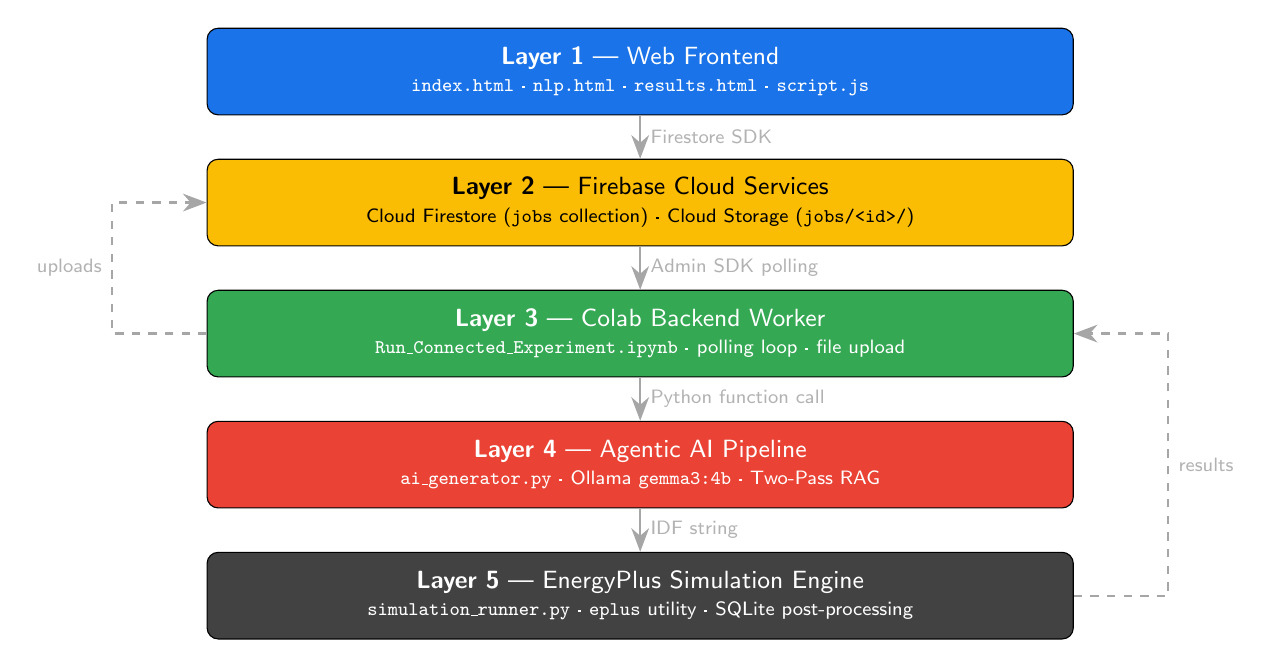
\begin{tikzpicture}[
  layer/.style={draw, rounded corners=4pt, minimum width=11cm, minimum height=1.1cm,
                font=\sffamily\small, text=white, align=center},
  arr/.style={-{Stealth[length=3mm]}, thick, gray!70},
  lbl/.style={font=\sffamily\scriptsize, gray!60},
]
  \node[layer, fill={rgb,255:red,26;green,115;blue,232}]                (L1) {\textbf{Layer 1} --- Web Frontend \\[-1pt] {\scriptsize\texttt{index.html} · \texttt{nlp.html} · \texttt{results.html} · \texttt{script.js}}};
  \node[layer, fill={rgb,255:red,251;green,188;blue,4}, text=black, below=0.55cm of L1]  (L2) {\textbf{Layer 2} --- Firebase Cloud Services \\[-1pt] {\scriptsize Cloud Firestore (\texttt{jobs} collection) · Cloud Storage (\texttt{jobs/<id>/})}};
  \node[layer, fill={rgb,255:red,52;green,168;blue,83}, below=0.55cm of L2]  (L3) {\textbf{Layer 3} --- Colab Backend Worker \\[-1pt] {\scriptsize\texttt{Run\_Connected\_Experiment.ipynb} · polling loop · file upload}};
  \node[layer, fill={rgb,255:red,234;green,67;blue,53}, below=0.55cm of L3]  (L4) {\textbf{Layer 4} --- Agentic AI Pipeline \\[-1pt] {\scriptsize\texttt{ai\_generator.py} · Ollama \texttt{gemma3:4b} · Two-Pass RAG}};
  \node[layer, fill={rgb,255:red,66;green,66;blue,66}, below=0.55cm of L4]  (L5) {\textbf{Layer 5} --- EnergyPlus Simulation Engine \\[-1pt] {\scriptsize\texttt{simulation\_runner.py} · \texttt{eplus} utility · SQLite post-processing}};

  \draw[arr] (L1) -- node[right, lbl]{Firestore SDK} (L2);
  \draw[arr] (L2) -- node[right, lbl]{Admin SDK polling} (L3);
  \draw[arr] (L3) -- node[right, lbl]{Python function call} (L4);
  \draw[arr] (L4) -- node[right, lbl]{IDF string} (L5);

  \draw[arr, dashed] (L5.east) -- ++(1.2,0) |- node[near start, right, lbl]{results} (L3.east);
  \draw[arr, dashed] (L3.west) -- ++(-1.2,0) |- node[near start, left, lbl]{uploads} (L2.west);
\end{tikzpicture}
\caption{Five-layer architecture stack and primary data channels.}
\label{fig:layers}
\end{figure}

% --- LAYER 1 ---
\subsection{Layer 1 --- Web Frontend}

The frontend is a static single-page application served locally via Python's built-in HTTP server (\texttt{python -m http.server 8000}). It consists of vanilla HTML, CSS, and JavaScript---no build step or framework is required.

\subsubsection{User Interface Pages}
\begin{itemize}[nosep]
  \item \texttt{nlp.html}: The user types a natural-language building description, selects an AI model (\texttt{openai}, \texttt{gemini}, \texttt{huggingface}, or \texttt{ollama}), and chooses a weather file. Clicking \emph{Submit} calls \texttt{submitDescription()} in \texttt{script.js}.
  \item \texttt{results.html}: Displays a table of all submitted jobs. Clicking a row calls \texttt{showJobDetails()}, which renders status badges, result plot images, and two action buttons: \emph{View Generated IDF} and \emph{View Object Summary}.
\end{itemize}

\subsubsection{Client Logic (\texttt{script.js})}
The script initialises Firebase using the credentials exported from \texttt{firebaseConfig.js}, then exposes the following key functions:
\begin{description}[nosep, leftmargin=1.5cm, labelwidth=1.3cm]
  \item[\texttt{submitDescription()}] Writes a new document to the Firestore \texttt{jobs} collection with \texttt{status: "queued"}.
  \item[\texttt{loadJobs()}] Reads all documents from \texttt{jobs}, sorts by timestamp, and populates the results table.
  \item[\texttt{showJobDetails()}] Fetches plot images from Firebase Storage using \texttt{storage.ref().getDownloadURL()} and sets them as \texttt{<img>} sources (images bypass CORS natively).
  \item[\texttt{viewIDF()}] Opens the backend-generated \texttt{diff.html} (a side-by-side diff of Base vs.\ Generated IDF) in a new tab.
  \item[\texttt{viewIDFSummary()}] Opens the backend-generated \texttt{summary.html} in a new tab, displaying all IDF objects in expandable accordion cards.
  \item[\texttt{testAIConnection()}] Writes a test document to Firestore's \texttt{test\_connectivity} collection and waits for the backend to respond.
\end{description}

% --- LAYER 2 ---
\subsection{Layer 2 --- Firebase Cloud Services}

Firebase acts as the stateless coordination bus between the browser and the Colab worker. Two services are used:

\begin{itemize}[nosep]
  \item \textbf{Cloud Firestore} --- A NoSQL document database. The \texttt{jobs} collection stores one document per simulation request. Fields include \texttt{status} (\texttt{queued} $\to$ \texttt{running} $\to$ \texttt{done} / \texttt{error}), \texttt{nlpInputText}, \texttt{simulationConfig}, and \texttt{resultPaths}.
  \item \textbf{Cloud Storage} --- Binary file storage. The backend uploads plot PNGs, the generated IDF, the HTML diff, and the HTML summary to the path \texttt{jobs/<jobId>/}.
\end{itemize}

No custom Cloud Functions or servers are deployed; the Colab notebook polls Firestore directly.

% --- LAYER 3 ---
\subsection{Layer 3 --- Colab Backend Worker}

The Jupyter notebook \texttt{Run\_Connected\_Experiment.ipynb} is executed on a Google Colab GPU runtime. Its cells perform the following boot sequence:

\begin{enumerate}[nosep]
  \item Mount Google Drive to access the repository files.
  \item Copy the pre-downloaded Ollama model weights from Drive to the Colab SSD (\texttt{/root/.ollama/models/}) for fast memory-mapped inference.
  \item Start the Ollama server with \texttt{nohup ollama serve} and wait for readiness.
  \item Initialise \texttt{FirebaseConnector} and \texttt{AIPipelines}.
  \item Enter an infinite polling loop that queries Firestore every 3~seconds for documents where \texttt{status == "queued"}.
\end{enumerate}

When a queued job is found, the loop:
\begin{enumerate}[nosep]
  \item Sets \texttt{status} to \texttt{"running"}.
  \item Calls \texttt{ai.generate\_idf\_from\_text()} to produce the IDF string (Layer~4).
  \item Saves the IDF to \texttt{RunFiles/<jobId>\_in.idf}.
  \item Calls \texttt{simulation\_runner.run\_simulation\_job()} to execute EnergyPlus (Layer~5).
  \item Uploads every result file (plots, CSV, IDF, \texttt{diff.html}, \texttt{summary.html}) to Firebase Storage.
  \item Sets \texttt{status} to \texttt{"done"} and writes \texttt{resultPaths}.
\end{enumerate}

% --- LAYER 4 ---
\subsection{Layer 4 --- Agentic AI Pipeline}

The AI pipeline lives in \texttt{backend/ai\_generator.py} inside the \texttt{AIPipelines} class. It supports four LLM backends: OpenAI, Google Gemini, HuggingFace Inference, and a local Ollama instance running \texttt{gemma3:4b}.

\subsubsection{Two-Pass Agentic RAG Workflow}

The core generation method \texttt{generate\_idf\_from\_text()} implements a Retrieval-Augmented Generation (RAG) pattern in two passes. Figure~\ref{fig:rag} illustrates the flow.

\begin{figure}[H]
\centering
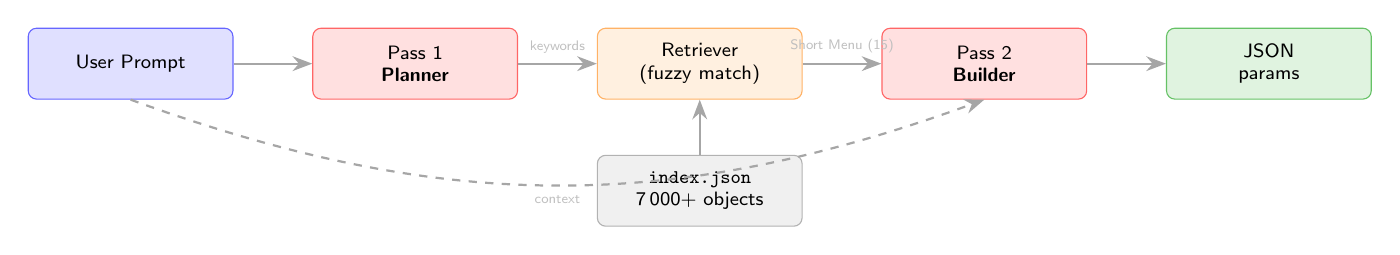
\begin{tikzpicture}[
  box/.style={draw, rounded corners=3pt, minimum height=0.9cm, minimum width=2.6cm,
              font=\sffamily\scriptsize, align=center, fill=#1!12, draw=#1!60},
  arr/.style={-{Stealth[length=2.5mm]}, thick, gray!70},
  data/.style={font=\sffamily\tiny, gray!50},
]
  \node[box=blue]  (prompt) {User Prompt};
  \node[box=red, right=1.0cm of prompt]   (p1) {Pass 1\\\textbf{Planner}};
  \node[box=orange, right=1.0cm of p1]    (ret) {Retriever\\(fuzzy match)};
  \node[box=red, right=1.0cm of ret]      (p2) {Pass 2\\\textbf{Builder}};
  \node[box=green!60!black, right=1.0cm of p2]   (json) {JSON\\params};

  \node[box=gray, below=0.7cm of ret]  (idx) {\texttt{index.json}\\7\,000+ objects};

  \draw[arr] (prompt) -- (p1);
  \draw[arr] (p1) -- node[above, data]{keywords} (ret);
  \draw[arr] (ret) -- node[above, data]{Short Menu (15)} (p2);
  \draw[arr] (p2) -- (json);
  \draw[arr] (idx) -- (ret);
  \draw[arr, dashed, bend right=20] (prompt.south) to node[below, data]{context} (p2.south);
\end{tikzpicture}
\caption{Two-pass Agentic RAG workflow inside \texttt{ai\_generator.py}.}
\label{fig:rag}
\end{figure}

\paragraph{Pass 1 --- The Planner.}
The method \texttt{\_generate\_search\_keywords()} sends the user's natural-language prompt to the LLM with instructions to return a JSON array of material and HVAC keywords. If the prompt is vague, the model is instructed to infer ASHRAE-standard defaults. The returned list typically contains 5--20 keywords such as \texttt{["wood stud", "brick", "insulation", "metal roof"]}.

\paragraph{The Retriever.}
The 7\,000+ entries in \texttt{index.json} (built by \texttt{dataset\_indexer.py}) are scored against the Planner's keywords using a simple fuzzy-matching function. The top 15 constructions form the \emph{Short Menu}.

\paragraph{Pass 2 --- The Builder.}
A second LLM call receives the user prompt together with the Short Menu and a strict JSON schema. The schema demands 15~keys covering geometry (\texttt{length}, \texttt{width}, \texttt{height}), envelope (\texttt{wall\_construction}, \texttt{roof\_construction}), windows (\texttt{wwr}, \texttt{window\_u\_factor}, \texttt{window\_shgc}), internal gains (\texttt{people\_density}, \texttt{light\_density}, \texttt{equipment\_density}), airflow (\texttt{ventilation\_ach}, \texttt{infiltration\_ach}), and setpoints (\texttt{heat\_set\_occ}, \texttt{heat\_set\_unocc}, \texttt{cool\_set\_occ}, \texttt{cool\_set\_unocc}).

\subsubsection{IDF Assembly}

After parsing the JSON response, the assembler:
\begin{enumerate}[nosep]
  \item Calls \texttt{geometry\_util.generate\_zone\_geometry(L, W, H, wwr)} to produce 3-D vertices for walls, roof, floor, and window sub-surfaces.
  \item Calls \texttt{idf\_extractor.resolve\_dependencies()} for the chosen wall and roof constructions. This recursively fetches the \texttt{Construction} block and all referenced \texttt{Material} blocks from the Datasets folder.
  \item Concatenates the parameterised \texttt{Base.idf} template, the extracted material blocks, and the geometry block.
  \item Performs placeholder injection: every \texttt{\{PLACEHOLDER\}} token in the combined string (e.g.,\ \texttt{\{PEOPLE\_DENSITY\}}, \texttt{\{COOL\_OCC\}}) is replaced with the AI-extracted numeric value.
\end{enumerate}

% --- LAYER 5 ---
\subsection{Layer 5 --- EnergyPlus Simulation Engine}

\texttt{simulation\_runner.py} wraps the \texttt{eplus} utility library (installed from a custom GitHub branch). Its \texttt{run\_simulation\_job()} function:

\begin{enumerate}[nosep]
  \item Calls \texttt{prepare\_colab\_eplus()} to ensure the EnergyPlus binary is available.
  \item Creates an \texttt{EPlusUtil} instance and configures the model, weather, and output directory.
  \item Runs the simulation (\texttt{design\_day} or \texttt{annual}).
  \item Opens the resulting SQLite database (\texttt{eplusout.sql}) with \texttt{EPlusSqlExplorer} and queries for output variables such as Zone Air Temperature, Cooling Energy, and Heating Energy.
  \item Generates \texttt{matplotlib} plots and saves them as PNGs.
  \item Parses the generated IDF text to produce \texttt{summary.html}---an HTML page with expandable accordion cards listing every EnergyPlus object and its detailed fields.
\end{enumerate}

% ==============================================================================
\section{End-to-End Data Flow}
% ==============================================================================

The complete lifecycle of a single simulation job is illustrated in Figure~\ref{fig:flow} and described step-by-step below.

\begin{figure}[H]
\centering
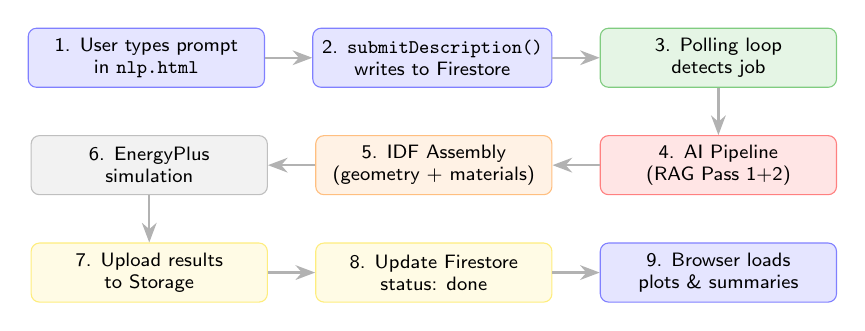
\begin{tikzpicture}[
  step/.style={draw, rounded corners=3pt, minimum height=0.75cm, minimum width=3.0cm,
               font=\sffamily\scriptsize, align=center, fill=#1!10, draw=#1!50},
  arr/.style={-{Stealth[length=2.5mm]}, thick, gray!60},
]
  \node[step=blue]   (s1) {1. User types prompt\\in \texttt{nlp.html}};
  \node[step=blue, right=0.6cm of s1]   (s2) {2. \texttt{submitDescription()}\\writes to Firestore};
  \node[step=green!60!black, right=0.6cm of s2]  (s3) {3. Polling loop\\detects job};

  \node[step=red, below=0.6cm of s3]    (s4) {4. AI Pipeline\\(RAG Pass 1+2)};
  \node[step=orange, left=0.6cm of s4]  (s5) {5. IDF Assembly\\(geometry + materials)};
  \node[step=gray, left=0.6cm of s5]    (s6) {6. EnergyPlus\\simulation};

  \node[step=yellow!80!orange, below=0.6cm of s6, text=black]   (s7) {7. Upload results\\to Storage};
  \node[step=yellow!80!orange, right=0.6cm of s7, text=black]   (s8) {8. Update Firestore\\status: done};
  \node[step=blue, right=0.6cm of s8]   (s9) {9. Browser loads\\plots \& summaries};

  \draw[arr] (s1) -- (s2);
  \draw[arr] (s2) -- (s3);
  \draw[arr] (s3) -- (s4);
  \draw[arr] (s4) -- (s5);
  \draw[arr] (s5) -- (s6);
  \draw[arr] (s6) -- (s7);
  \draw[arr] (s7) -- (s8);
  \draw[arr] (s8) -- (s9);
\end{tikzpicture}
\caption{End-to-end lifecycle of a single simulation job.}
\label{fig:flow}
\end{figure}

\begin{enumerate}[nosep]
  \item \textbf{User $\to$ Browser}: Types a building description into \texttt{nlp.html}.
  \item \textbf{Browser $\to$ Firestore}: \texttt{submitDescription()} writes a document with \texttt{status:"queued"} to the \texttt{jobs} collection.
  \item \textbf{Colab $\leftarrow$ Firestore}: The polling loop detects the queued document and marks it \texttt{"running"}.
  \item \textbf{Colab $\to$ Ollama}: Pass~1 extracts keywords; the Retriever filters \texttt{index.json}; Pass~2 returns a JSON parameter dictionary.
  \item \textbf{Colab (Assembly)}: \texttt{geometry\_util} + \texttt{idf\_extractor} + \texttt{Base.idf} $\to$ complete IDF string with injected values.
  \item \textbf{Colab $\to$ EnergyPlus}: \texttt{simulation\_runner} executes the IDF against the \texttt{.epw} weather file.
  \item \textbf{Colab $\to$ Storage}: Plots, CSV, IDF, \texttt{diff.html}, and \texttt{summary.html} are uploaded to Firebase Storage.
  \item \textbf{Colab $\to$ Firestore}: Document updated to \texttt{status:"done"} with \texttt{resultPaths}.
  \item \textbf{Browser $\leftarrow$ Firestore/Storage}: \texttt{loadJobs()} refreshes the table; \texttt{showJobDetails()} loads plot images; buttons open the IDF diff and object summary.
\end{enumerate}

% ==============================================================================
\section{Key Design Decisions}
% ==============================================================================

\begin{itemize}[nosep]
  \item \textbf{Serverless coordination}: Firebase eliminates the need for a dedicated backend server. The Colab notebook acts as an ephemeral worker that can be started and stopped without infrastructure changes.
  \item \textbf{Local LLM on Colab GPU}: Running \texttt{gemma3:4b} via Ollama on the Colab T4 GPU avoids per-token API costs and removes internet-latency from the generation loop. Model weights are persisted on Google Drive and copied to the SSD at boot to satisfy Ollama's memory-mapping requirements.
  \item \textbf{Agentic RAG}: The two-pass design prevents context-window overflow. Pass~1 reduces 7\,000+ objects to 15, enabling Pass~2 to focus on precise parameter extraction.
  \item \textbf{Template + Injection}: Rather than asking the LLM to write raw IDF syntax (error-prone), the system uses a human-verified \texttt{Base.idf} with placeholder tokens. The LLM only outputs structured JSON; all IDF syntax is handled deterministically.
  \item \textbf{CORS avoidance}: Plot images use \texttt{<img>} tags (exempt from CORS). The IDF summary is pre-rendered as \texttt{summary.html} on the backend and opened via \texttt{window.open()}, bypassing the browser's cross-origin \texttt{fetch} restrictions entirely.
\end{itemize}

% ==============================================================================
\section{Conclusion}
% ==============================================================================

SmartHVAC Studio demonstrates a feasible pipeline for translating natural-language building descriptions into validated EnergyPlus simulations. The five-layer separation of concerns allows each component---browser UI, cloud database, GPU worker, LLM intelligence, and physics engine---to evolve independently. The Agentic RAG approach, combined with deterministic template injection, achieves a practical balance between AI flexibility and simulation reliability.

\end{document}
